\chapter{Introduction} \label{chap:introduction}
\section{Overview} \label{sec:introduction_overview}
The \textit{standard model} (SM; sec.~\ref{sec:introduction_standard_model}) of particle physics is our current best mathematical framework for describing the behavior
of elementary particles. The domain of applicability of the SM is quite substantial, encompassing
every well-measured fundamental interaction of every verified fundamental particle. All SM particles have been conclusively observed,
and no fundamental particles outside the SM have ever been conclusively observed. After decades of effort by thousands of researchers,
no significant deviation from SM predictions has ever been confirmed in high-energy scattering experiments~\cite{ref:CahnGoldhaber, ref:PDG}.
These efforts are extended here with studies of the relationship between two particles, \PZ\ and \Pgamma, at state-of-the-art precision
(sec.~\ref{sec:introduction_znng} and~\ref{sec:introduction_aTGC}).

There are nevertheless many physical phenomena that the SM does not account for, such as the nature of gravitation (sec.~\ref{sec:introduction_ADD}),
including the gravitational phenomenon known as \textit{dark matter} (DM; sec.~\ref{sec:introduction_dm}). Many theories of physics beyond the SM (BSM)
have been developed in an attempt to describe these phenomena.

Specifically, this thesis presents several analyses of event yields in \textit{monophoton} final states, characterized by a single \Pgamma\ with
high transverse momentum, along with an overall transverse momentum imbalance typically of equal magnitude and opposite direction to
that of the \Pgamma. These analyses correspond to 35.9\fbinv\ of 13\unit{TeV} proton--proton (\Pp\Pp) collision data collected in 2016 by the CMS
detector at the LHC.

\section{Standard model of particle physics} \label{sec:introduction_standard_model}
The set of particles described by the SM is illustrated in Fig.~\ref{fig:sm_particles}, which
groups them according to certain fundamental characteristics.
Each particle has an intrinsic angular momentum known as \text{spin}, specified by the lower number in each square of Fig.~\ref{fig:sm_particles}.
Spin can be an integer or half-integer, according to which the particle is classified as a \textit{boson} or \textit{fermion}, respectively.
The fundamental fermions comprise six ``flavors'' of quarks---up (\Pu), down (\Pd), charm (\Pc), strange (\Ps), top (\Pt), and bottom (\Pb)---and six flavors of
leptons: electron (\Pe), muon (\Pmu), and tau (\Ptau), with three corresponding neutrinos (\Pne, \Pnmu, \Pntau).
Each of these has both a particle and an anti-particle variety; the quarks additionally come in three ``colors''.
We typically denote a particle by a letter, e.g. \Pq\ for a generic quark; its antiparticle partner has an overbar, e.g. \Paq.
The fundamental bosons comprise the \PH\ as well as the gauge bosons, in turn comprising the \PZ, photon (\Pgamma),
two \PW s distinguished by their electric charge, and eight gluons (\Pg) distinguished by a color-anticolor doublet.

\begin{figure}[hbtp]
  \begin{center}
    \includegraphics[width=1.0\textwidth]{Figures/sm_particles.png}
    \caption{
      The particles of the Standard Model.
    }
    \label{fig:sm_particles}
  \end{center}
\end{figure}

The particles are related to one another through various
classes of interactions, each of which has a corresponding charge whose sum must be conserved in any physical process.
The electromagnetic and weak interactions correspond to electric charge and weak isospin, respectively.
In Fig.~\ref{fig:sm_particles}, the value $Q$ of the electric charge is specified by the middle number in each square.
For quarks and leptons, weak isospin determines whether the particle is ``up-type''
(\Pu, \Pd, \Pt, \Pne, \Pnmu, \Pntau) or ``down-type'' (\Pd, \Ps, \Pb, \Pe, \Pmu, \Ptau).
Weak isospin has a corresponding value $T_{3}$: up-type fermions have $T_{3} = \mathrm{+}1/2$, down-type fermions and the \PH\ have
$T_{3} = \mathrm{-}1/2$, $W^\pm$ have $T_{3} = \pm1$, and the other bosons have $T_{3} = 0$.
The three colors carried by quarks and gluons are associated with the strong interaction, described by the theory of \textit{quantum
chromodynamics} (QCD). The preceding discussion applies to normal (i.e.\ not anti-) particles; antiparticles carry opposite values of all the
aforementioned charges.

These interactions lead to the relationships illustrated in Fig.~\ref{fig:sm_interactions}, in which every linkage represents
a direct \textit{coupling}, which allows a particle at one end of the link to evolve directly into a particle at the other end.
Particles with a nonzero electric charge are all coupled directly to the photon. The photon is coupled to the weak bosons
(\PZ\ and $W^\pm$), which in turn couple to all of the fundamental fermions. The gluons couple directly with each other and with the quarks.
Particles that couple directly to the \PH\ have an intrinsic mass (specified by the top number in each square of Fig.~\ref{fig:sm_particles}\footnote{The
proper units of mass are $\mathrm{GeV}\,c^{2}$, but the factor of $c^{2}$ is often omitted for brevity. This is done even when units of distance and
time (such as cm and ns) are used in which $c$ does not equal 1. Similarly, the factor of $1/c$ is often omitted from the proper units of momentum,
$\mathrm{GeV}/c$. This is the convention followed in this thesis.}) tied to the strength of their coupling.
In the SM, any particle that does not couple directly to the \PH\ is massless.

\begin{figure}[hbtp]
  \begin{center}
    \includegraphics[width=0.7\textwidth]{Figures/Elementary_particle_interactions_in_the_Standard_Model.png}
    \caption{
      Standard Model couplings.
    }
    \label{fig:sm_interactions}
  \end{center}
\end{figure}

The full dynamics of the SM is encapsulated mathematically by a \textit{Lagrangian} function. Particles correspond to operator
terms appearing in the Lagrangian, and a coupling of one particle to another is described by multiplying their
corresponding operators together. The SM Lagrangian is unchanged
if all its fermion operators are multiplied by any complex number of the form $e^{iY\theta}$, where the \textit{hypercharge} $Y$ is a value that depends
on the operator being multiplied. The is true even if $\theta$ is allowed to have different arbitrary values at
different points in space and time, but any operator with a nonzero $Y$ couples to an additional spin-1 operator denoted by \PB,
and as a consequence the first derivatives of $\theta$ in space and time must also be subtracted from \PB.
This deep level of invariance is called a \textit{gauge symmetry}, with \PB\ the associated \textit{gauge boson}.
Multiplication by $e^{i\theta}$ is characterized by the group $U(1)$, so we say that the SM Lagrangian has a
$U(1)_{Y}$ gauge symmetry associated with the \PB.

In a similar vein, the SM Lagrangian is unchanged if matching doublets
of weak isospin up- and down-type operators are multiplied by unitary $2\times2$ matrices with determinant 1, described by the
group $SU(2)$. Those with a nonzero weak isospin couple to every $W^{i}$ ($i=1,2,3$), which must receive their own balancing transformations
if the fermion $SU(2)$ transformations are allowed to vary as a function of space and time.
Hence we say that the SM Lagrangian has an $SU(2)$ gauge symmetry associated with the gauge bosons $W^{i}$.

The \PB\ and $W^{i}$s also couple to the \PH, and the structure of this coupling constrains the physical states
most easily accessed by these operators, corresponding to four distinct linear combinations of
\PB\ and $W^{i}$. These combinations, which are themselves operators, are labeled \PZ, \Pgamma, \PWplus, and \PWminus,
and these are the operators describing the physical particles detected in experiments.
In this manner, the electromagnetic and weak interactions are intertwined into the \textit{electroweak} (EWK) interaction.
The conserved electric charge $Q$ emerges as the sum of $T_{3}$ with $\frac{1}{2}Y$.

Finally, the SM Lagrangian has an additional $SU(3)$ gauge symmetry associated with the eight gluons and color charge, described by QCD.
Particles with color charge do not exist stably on their own, but rather are always observed in bound states called \textit{hadrons}, in which the overall color
charge state is invariant under any $SU(3)$ transformation. One such ``colorless'' configuration is the proton (\Pp), which
to a first approximation may be thought of as a bound state of two $u$ quarks and one $d$ quark.

However, the mass of the proton is much greater than the sum of the masses of these three components, and this additional mass is associated with an effervescent
``sea'' of \textit{partons}, transient particles swarming the proton that can only be distinguished at high energies.
Known partons include gluons (carrying about 50\% of the total momentum of a high-energy proton),
all types of quark and antiquark, and photons. As a consequence, a high-energy collision between two protons can give rise to a $q\bar{q}$ interaction,
which is the primary catalyst for all the processes studied below. A single parton carries some fraction of the total energy carried by the whole proton,
so in general, partons collide with a lower interaction energy than that of the protons that carry them.
The square of the center-of-mass energy of colliding protons is denoted by $s$, while that of a specific
parton-parton interaction is denoted by $\hat{s}$.

This rapid overview of the SM necessarily elides many essential nuances of the underlying mathematical formalism. These are more fully
documented in numerous comprehensive texts on the subject, e.g.~\cite{ref:HalzenMartin, ref:BargerPhillips, ref:PeskinSchroeder, ref:Srednicki, ref:Schwartz}.

\section{\texorpdfstring{\zinvg}{Z(νν)γ} cross section} \label{sec:introduction_znng}
In a collision of two beams of particles, the average rate of any specific collision process is directly proportional to the
number of particles in each of the colliding beams, to their density in the plane transverse to the beam direction, and to the average
frequency at which particles are made to come into contact. These features determine the instantaneous \textit{luminosity} $\mathcal{L}$ of a pair
of colliding beams, and the overall average rate of a given process may be written as $\sigma \mathcal{L}$, where $\sigma$
is a constant of proportionality. Since $\sigma$ has dimensions of area, it is called the \textit{cross section}.

Cross sections may be calculated using \textit{Feynman diagrams}. These are
assembled by combining fundamental interaction vertices: the SM vertices relating the fermions and gauge bosons are listed in Fig.~\ref{fig:sm_vertices}.
Mathematical terms are assigned to Feynman diagrams according to a prescription known as the Feynman rules, which can be derived from the Lagrangian.
This process results in a \textit{matrix element} $\mathcal{M}_{i}$ for each diagram $i$ one wishes to consider. The cross section is proportional to the sum of $|\sum_{i}{\mathcal{M}_{i}}|^{2}\rho$
over all kinematically consistent initial and final states of the given process\footnote{$\rho$ is a function of the allowed kinematic parameters and is called the \textit{phase space
factor}.}. This method for calculating cross sections using Feynman diagrams is more fully described in refs.~\cite{ref:HalzenMartin, ref:BargerPhillips};
a development in the context of quantum field theory is given in e.g. refs.~\cite{ref:PeskinSchroeder, ref:Srednicki, ref:Schwartz}.

\begin{figure}[hbtp]
  \begin{center}
    \includegraphics[width=0.7\textwidth]{Figures/Standard_Model_Feynman_Diagram_Vertices.png}
    \caption{
      Fermion and gauge boson vertices of the standard model.
    }
    \label{fig:sm_vertices}
  \end{center}
\end{figure}

The Feynman rule for a vertex includes a coupling constant $g$. These are typically less than 1 in high-energy collisions, meaning diagrams
with additional vertices make smaller contributions to a cross section calculation. Whenever this is the case, we say that
$|\sum_{i}{\mathcal{M}_{i}}|^{2}$ admits a \textit{perturbative expansion}, in which the expression is organized as a sum of terms with increasing powers
of $\alpha \propto g^{2}$, which make successively smaller contributions.
Terms with the lowest powers of $\alpha$ are called leading order (LO) terms, followed by next-to-leading order (NLO), next-to-next-to-leading order (NNLO), etc.
Diagrams with an internal loop contain at least one more vertex than equivalent diagrams without the loop, and therefore \textit{tree-level} diagrams without any internal loops
make the only contributions at LO (when they exist). Each class of interaction has its own characteristic coupling constant:
an $\alpha$ without a subscript usually refers to the fine structure constant characterizing electromagnetic processes, while QCD is characterized by the strong coupling $\alpha_\mathrm{S}$.

In the SM, events with a monophoton signature arise at the LHC (Chap.~\ref{chap:LHCCMS}) primarily from the process $q\bar{q} \to \PZ\Pgamma \to \Pn\Pan\Pgamma$,
where $q$ is any single species of quark, \Pn\ is any single species of neutrino, and the neutrino-antineutrino pair arises from the decay
of a short-lived \PZ\ boson. The leading tree-level diagram for this process is shown in Fig.~\ref{fig:zinvg_diagrams}(a). We typically abbreviate this process by
reference to its final state, \zinvg. The final-state photon can be detected, but the neutrinos only interact with SM particles via the mediation
of \PZ\ and \PW\ bosons, and these interactions are strongly suppressed by the high masses of those particles. Hence, neutrinos almost never interact directly with the LHC's detectors.

\begin{figure}[htb]
  \begin{center}
    \includegraphics[width=0.49\textwidth]{Figures/zg_isr_v11.pdf}
    \includegraphics[width=0.49\textwidth]{Figures/zg_zzg_v11.pdf}
    \includegraphics[width=0.49\textwidth]{Figures/zg_zgg_v11.pdf}
    \caption{
      The leading Feynman diagrams for \zinvg\ production arising from \Pp\Pp\ collisions. Diagram (a) is the leading SM contribution.
      Diagrams (b) and (c) show contributions from aTGC vertices.
    }
    \label{fig:zinvg_diagrams}
  \end{center}
\end{figure}

Their existence is instead inferred by their absence.
In a collider experiment, the vectorial momentum transverse to the beam direction, \vecpT, must sum to approximately zero in the reference frame of the
detector. The negative vector sum of \vecpT\ for all detected particles in an event is denoted \vecMET, and its magnitude \MET\ must therefore be close
to zero if all the particles in an event are reliably detected and their momenta are accurately measured. The only high-momentum SM particles that can't
be reliably detected are neutrinos, so a large value of \MET\ can be a sign of neutrino production. An event with a high-\pT\ detected photon, in which
the \vecMET\ has a large magnitude and points in a direction significantly different from that of the photon, is called a monophoton event, and it is
expected that \zinvg\ processes are the main contributors of high-\pT\ monophoton events.

The theoretical SM value for the \zinvg\ cross section has been calculated to NLO in $\alpha$ and $\alpha_\mathrm{S}$~\cite{ref:JHEP04(2015)018, ref:JHEP02(2016)057}.
The \zinvg\ process receives NLO contributions from 1-loop QCD and EWK diagrams, as well as tree-level diagrams with up to one additional radiated \Pgamma, \Pq, or \Pg.
These contributions include diagrams with initial-state \Pq\Paq, \Pq\Pg, and \Paq\Pg\ (with QCD and EWK corrections at NLO), as well as \Pq\Pgamma, \Paq\Pgamma\ (with EWK corrections
at NLO)~\cite{ref:JHEP02(2016)057}.

The calculation has also been done to NNLO in $\alpha_\mathrm{S}$ alone,
which includes contributions from tree-level diagrams with up to two extra radiated QCD partons (\Pq\ or \Pg), one-loop diagrams with up to one extra
radiated QCD parton, and two-loop corrections. The initial-state QCD parton interactions include those listed among the NLO contributions above,
as well as $gg$~\cite{ref:j.physletb.2014.02.037, ref:JHEP07(2015)085}.

The exact values obtained from any such calculation depend on the specific initial and final states included. These restrictions (\textit{cuts}) on events are
informed by the operating conditions of the experiment one wishes to compare results with.

\subsection{Previous measurements} \label{sec:introduction_znng_previous_measurements}
Experiments at the LEP detector measured the cross section of \zinvg\ arising from $e^{\mathrm{+}}e^{\mathrm{-}}$ collisions for $\sqrt{s}$ up to \textasciitilde200 GeV.
The L3 experiment measured the cross section to be $5.1 \pm 0.3\mathrm{(stat)} \pm 0.1\mathrm{(syst)}$ $pb$ based on 175.6 $pb^{-1}$ of collision data with an average $\sqrt{s} = 188.6$ GeV, compared to an SM
prediction of $4.99 \pm 0.05\mathrm{(stat)}$~\cite{ref:j.physletb.2004.07.002}. Looking at collision data at the same $\sqrt{s}$, but with different cuts,
the OPAL experiment measured the cross section to be $2.52 \pm 0.13\mathrm{(stat)} \pm 0.05\mathrm{(syst)}$ $pb$ based on 177.3 $pb^{-1}$ of data, compared to an SM
prediction of $2.81 \pm 0.02\mathrm{(stat)}$ $pb$~\cite{}. This set of SM predictions were made up to $O(\alpha^2)$, but LO in $\alpha_\mathrm{S}$.

The D0 experiment at the Tevatron made the first observation of \zinvg\ arising from $p\bar{p}$ collisions in 2009. This yielded a cross section measurement of
$32 \pm 9\mathrm{(stat+syst)} \pm 2\mathrm{(lumi)}$ $fb$ for a leading photon \pT\ above 90\unit{GeV}\footnote{The proper units for momentum are $\mathrm{GeV}/c$, but the
factor of $c$ is often omitted for brevity, and this is the convention followed in this thesis. Similarly, the proper units for mass are $\mathrm{GeV}\,c^{2}$, but the factor
of $c^{2}$ is usually omitted.},
compared to an SM prediction of $39 \pm 4\mathrm{(theory)}$ $fb$ computed to NLO in $\alpha_\mathrm{S}$~\cite{ref:PhysRevLett.102.201802}.

Measurements of the cross section at higher values of \pTgamma\ have been performed by experiments examining \Pp\Pp\ collision data at the LHC.
An analysis by the CMS experiment examining 19.6\fbinv\ of data collected at $\sqrt{s} = 8\unit{TeV}$ found the observed \zinvg\ cross section for $\pTgamma > 145\unit{GeV}$ to be
$52.7 \pm 2.1\mathrm{(stat)} \pm 6.4\mathrm{(syst)} \pm 1.4\mathrm{(lumi)}$ $fb$, compared to an SM prediction of $40.7 \pm 4.9\mathrm{(theory)}$ $fb$ calculated to NLO in $\alpha_\mathrm{S}$, and
a prediction of $50.0^{+2.4}_{-2.2}\mathrm{(theory)}$ calculated to NNLO in $\alpha_\mathrm{S}$~\cite{ref:j.physletb.2016.06.080}. This comparison illustrates the need for NNLO precision at high \pTgamma.

The most precise measurement of the \zinvg\ cross section for \pTgamma\ and \MET\ above 150\unit{GeV} currently comes from an analysis of 36.1\fbinv\ of \Pp\Pp\ collision data
collected by the ATLAS experiment at $\sqrt{s} = 13\unit{TeV}$, with an observed cross section of $83.7^{+3.6}_{-3.5}\mathrm{(stat)}^{+6.9}_{-6.2}\mathrm{(syst)}^{+1.7}_{-2.0}\mathrm{(lumi)}$ $fb$.
The corresponding SM prediction, computed to NNLO in $\alpha_\mathrm{S}$ using the MATRIX generator~\cite{ref:epjc/s10052-018-5771-7}, is $78.6 \pm 0.4\mathrm{(stat)} \pm 4.1\mathrm{(syst)}$ $fb$~\cite{ref:CERN-EP-2018-220}.
The cross section is shown in discrete ranges (bins) of leading photon \pT\ in Fig.~\ref{fig:znng_xsec_phoET_ATLAS}.

\begin{figure}[hbtp]
  \begin{center}
    \includegraphics[width=0.4\textwidth]{Figures/znng_xsec_phoET_ATLAS.png}
    \caption{
      Cross section of \zinvg\ production plotted in bins of leading photon \pT\ ($E^{\gamma}_\mathrm{T}$), as shown in~\cite{ref:CERN-EP-2018-220}.
      The blue and green bands show the SM predictions derived from the Sherpa~\cite{ref:1126-6708/2009/02/007} and MCFM~\cite{ref:JHEP07(2011)018} generators, respectively.
    }
    \label{fig:znng_xsec_phoET_ATLAS}
  \end{center}
\end{figure}

None of these analyses report any significant deviation from the SM predictions.

\section{Anomalous triple gauge couplings} \label{sec:introduction_aTGC}
Putative vertices joining three gauge bosons that are not found in the SM are known as \textit{anomalous triple gauge couplings} (aTGCs).
For example, there is no fundamental SM vertex joining a single \Pgamma\ to a pair of \PZ s, or a single \PZ\ to a pair of \Pgamma s. A model
describing the generic phenomenology of these aTGCs is developed in~\cite{ref:Nucl.Phys.0550-3213_87_90685-7, ref:PhysRevD.47.4889, ref:PhysRevD.62.113011}.
For an intermediate state $V = \PZ,\Pgamma$ decaying to a final state \PZ\Pgamma\ pair, this model parametrizes the effective vertex interaction $\PZ V\Pgamma$
by a set of factors $h_{i}^{V}$ ($i$ from 1 to 4). Increasing the values of these parameters significantly increases the cross section
of \zinvg\ processes, by allowing the reaction to proceed via the additional diagrams shown in Fig.~\ref{fig:zinvg_diagrams}(b),(c),
in which the aTGC vertices are covered by opaque circles.

The circle could be thought of as masking a more detailed process taking place underneath. The SM admits processes that are predicted to contribute
to this effective vertex, but all SM contributions to $h_{3,4}^{V}$ have at least one internal loop that could fit within the circle, and
further loops are required for $h_{1,2}^{V}$ contributions~\cite{ref:PhysRevD.47.4889}.
As a consequence, the SM contribution to all eight $h_{i}^{V}$ parameters is quite close to zero.
The observation of a substantial nonzero value for any $h_{i}^{V}$ would be a compelling sign of BSM physics.

The contributions to the \zinvg\ cross section coming from $h_{1,2}^{V}$ are independent of those from $h_{3,4}^{V}$ (for any $V$), and also nearly identical
in magnitude, so without loss of generality we only focus on scenarios for which $h_{3,4}^{V}$ are nonzero. The contributions
from $h_{i}^{\PZ}$ are largely independent of those from $h_{j}^{\Pgamma}$ (for any $i$,$j$), so these are examined separately.
However, the contributions from $h_{3}^{V}$ are substantially correlated with those from $h_{4}^{V}$ (and similarly for $h_{1,2}^{V}$), so we examine
scenarios in which $h_{3,4}^{V}$ take on assorted pairs of values, both of which may be nonzero. The theoretical relationships between these parameters
are explored in~\cite{ref:PhysRevD.47.4889}.

The neutrino decays of \PZ-bosons offer an especially good window on \PZ\PZ\Pgamma\ and \PZ\Pgamma\Pgamma\ aTGCs because the
probability that a \PZ\ will decay into neutrinos is about six times higher than that of a decay into $e^\mathrm{+}e^\mathrm{-}$, or into $\mu^\mathrm{+}\mu^\mathrm{-}$.
Furthermore, the probability of reconstructing a \zinvg\ event in a detector is typically
higher than that of a charged lepton event. As a consequence, aTGC limits derived from neutral \PZ\ decays can be several times
stronger than limits derived from charged \PZ\ decays when analyzing the same \Pp\Pp\ collision data sets (compare e.g.~\cite{ref:PhysRevD.89.092005} and~\cite{ref:JHEP10(2013)164},
based on 7\unit{TeV} LHC data; also Fig.~\ref{fig:lhc_8tev_atgc_1dlimits}, based on 8\unit{TeV} data).
The decays of \PZ\ into \Pq\Paq\ (and thence to hadrons) are difficult to distinguish in practice from hadronic \PW\ decays~\cite{ref:RevModPhys.89.035008}.

\subsection{Previous searches} \label{sec:introduction_aTGC_previous_searches}
The LEP collider established constraints on each of the eight the parameters $h_{i}^{V}$ in the context of the process $e^{\mathrm{+}}e^{\mathrm{-}} \to \PZ\Pgamma$.
In a statistical combination of searches perfomed by the DELPHI, L3, and OPAL experiments, examining 3\fbinv\ of $e^{\mathrm{+}}e^{\mathrm{-}}$ collision data
for $\sqrt{s}$ ranging from 130 GeV to 209 GeV, the 95\% CL intervals of seven of the parameters contain 0, with total ranges between 0.05 and 0.10 for $h_{i}^{\Pgamma}$
and between 0.14 and 0.25 for $h_{i}^{\PZ}$; the 95\% CL interval for the remaining factor $h_{4}^{\Pgamma}$ spans 0.01 to 0.05~\cite{ref:j.physrep.2013.07.004}.

The LEP combined analysis assumed that all but one of the eight parameters were fixed to the SM expectation of 0 (i.e.\ these are 1D limits).
It was also the last major effort to obtain limits on $h_{1,2}^{V}$ independently of $h_{3,4}^{V}$,
as subsequent searches have taken the present approach of focusing on $h_{3,4}^{V}$ alone, for the reasons listed above.
Uniquely among the LEP experiments, the L3 Collaboration also placed limits on correlated pairs of parameters (2D limits), shown in Fig.~\ref{fig:L3_atgc_contours}~\cite{ref:j.physletb.2004.07.002}.

\begin{figure}[hbtp]
  \begin{center}
    \includegraphics[width=0.8\textwidth]{Figures/L3_atgc_contours.jpg}
    \caption{
      $h_{i}^{V}$ exclusion contours from the L3 experiment at the LEP collider, as shown in~\cite{ref:j.physletb.2004.07.002}.
    }
    \label{fig:L3_atgc_contours}
  \end{center}
\end{figure}

Experiments at the Tevatron collider improved these limits in analyses of \Pp\Pap\ collision data at $\sqrt{s} = 1.96\unit{TeV}$.
The Tevatron analyses incorporated a form factor $1 / (1 + \hat{s}/\Lambda^{2})^{n}$, by which a constant term $h_{0i}^{V}$ is
multiplied to obtain $h_{i}^{V}$.
The form factor is essentially arbitrary; $n$ is set equal to $i$ and $\Lambda$ (not to be confused with the EFT suppression scale, below)
is set to 1.5\unit{TeV} by convention. This form factor was introduced in the common reference~\cite{ref:PhysRevD.47.4889} but was not used in LEP~\cite{ref:j.physrep.2013.07.004}
or most subsequent LHC analyses, which treat the $h_{i}^{V}$ parameters as constants independent of $\hat{s}$.

The CDF experiment combined analyses of \zinvg\ processes, using 4.9\fbinv\ of data, and processes where the \PZ\ decays to
$l^\mathrm{+}l^\mathrm{-}$ ($e^\mathrm{+}e^\mathrm{-}$ or $\mu^\mathrm{+}\mu^\mathrm{-}$), using 5.1\fbinv\ of data.
They set 95\%\ Bayesian credibility intervals constraining $|h_{3}^{V}| < 0.022$ and $|h_{4}^{V}| < 0.0009$ (1D limits)~\cite{ref:PhysRevLett.107.051802}.
The D0 experiment similarly combined a 3.6\fbinv\ \zinvg\ analysis with a 7.2\fbinv\ $Z(l^\mathrm{+}l^\mathrm{-})\gamma$
analysis to set 95\%\ CL limits constraining
$|h_{03}^{V}| < 0.027$ and $|h_{04}^{V}| < 0.0014$ (1D limits)~\cite{ref:PhysRevD.85.052001}. Correlated 2D limits were also
computed and are shown in Fig.~\ref{fig:d0_aTGC}.

\begin{figure}[hbtp]
  \begin{center}
    \includegraphics[width=0.45\textwidth]{Figures/d0_ZZg.png}
    \includegraphics[width=0.45\textwidth]{Figures/d0_Zgg.png}
    \caption{
      $h_{0i}^{V}$ exclusion contours from the D0 experiment at the Tevatron collider, from~\cite{ref:PhysRevD.85.052001}.
    }
    \label{fig:d0_aTGC}
  \end{center}
\end{figure}

Experiments at the LHC made further improvements via the analysis of \Pp\Pp\ collision data at progressively higher $\sqrt{s}$.
A summary of 1D limits on $h_{i}^{V}$ from both the ATLAS and CMS experiments obtained from analyses of \textasciitilde20\fbinv\ of $\sqrt{s} = 8\unit{TeV}$ data
is shown in Fig.~\ref{fig:lhc_8tev_atgc_1dlimits}. ATLAS limits show the results of combined \zinvg\ and $Z(l^\mathrm{+}l^\mathrm{-})\gamma$
analyses, both with and without a form factor on $h_{i}^{V}$. CMS limits show separate \zinvg\ results, along with $Z(l^\mathrm{+}l^\mathrm{-})\gamma$
results, both without a form factor~\cite{ref:RevModPhys.89.035008}. These comparisons make clear that \zinvg\ is by far
the more sensitive channel for setting aTGC limits.

\begin{figure}[hbtp]
  \begin{center}
    \includegraphics[width=\textwidth]{Figures/lhc_8tev_atgc_1dlimits.png}
    \caption{
      1D $h_{i}^{V}$ exclusion limits from the ATLAS and CMS experiments at the LHC based on 20\fbinv\ of $\sqrt{s} = 8\unit{TeV}$
      \Pp\Pp\ collision data, from~\cite{ref:RevModPhys.89.035008}.
      $Z\gamma(ll\gamma)$ indicates a combination of $Z(e^\mathrm{+}e^\mathrm{-})\gamma$ and $Z(\mu^\mathrm{+}\mu^\mathrm{-})\gamma$
      analyses; $Z\gamma(ll\gamma,\nu\nu\gamma)$ indicates a combination of these with \zinvg. The mass $\Lambda_{FF}$
      is the form factor scale; $\infty$ means no form factor was used.
    }
    \label{fig:lhc_8tev_atgc_1dlimits}
  \end{center}
\end{figure}

The most sensitive published limits on $h_{3,4}^{Z,\gamma}$ are currently derived from 36.1\fbinv\ of 13\unit{TeV} \Pp\Pp\ collision
data collected by the ATLAS detector at the LHC, analyzed exclusively in the monophoton channel, with no form factor~\cite{ref:CERN-EP-2018-220}.
These are summarized in Figs.~\ref{fig:atlas_atgc_13tev_1dlimits},~\ref{fig:atlas_atgc_13tev_2dlimits}.

\begin{figure}[hbtp]
  \begin{center}
    \includegraphics[width=0.8\textwidth]{Figures/atlas_atgc_13tev_1dlimits.png}
    \caption{
      1D $h_{i}^{V}$ exclusion limits from the ATLAS experiment at the LHC based on 36.1\fbinv\ of $\sqrt{s} = 13\unit{TeV}$
      \Pp\Pp\ collision data, analyzed in the monophoton channel, as shown in~\cite{ref:CERN-EP-2018-220}.
    }
    \label{fig:atlas_atgc_13tev_1dlimits}
  \end{center}
\end{figure}

\begin{figure}[hbtp]
  \begin{center}
    \includegraphics[width=\textwidth]{Figures/atlas_atgc_13tev_2dlimits.png}
    \caption{
      2D $h_{i}^{V}$ exclusion contours from the ATLAS experiment at the LHC based on 36.1\fbinv\ of $\sqrt{s} = 13\unit{TeV}$
      \Pp\Pp\ collision data, analyzed in the monophoton channel, as shown in~\cite{ref:CERN-EP-2018-220}.
    }
    \label{fig:atlas_atgc_13tev_2dlimits}
  \end{center}
\end{figure}

None of these analyses report any significant evidence of BSM physics.

\section{Dark matter EFT and simplified models} \label{sec:introduction_dm}
The standard theory of gravitation, Einstein's
general theory of relativity (GR), has passed experimental tests over scales ranging from the orbits of satellites~\cite{ref:lrr-2003-1} to the entire observable universe~\cite{ref:planck2018_cosparams},
matching observations more closely than Newton's theory of gravitation, to which it converges in the weak-field limit~\cite{ref:WaldGR}.
It predicts the existence of gravitional waves, directly detected for the first time in 2015~\cite{ref:PhysRevLett.116.061102}, and these have been used to test the theory in the strong-field regime~\cite{ref:PhysRevLett.116.221101}.

Despite its many triumphs, GR fails---under the assumption that SM particles and their known interactions are the only sort that exist---to describe the orbits of stars in nearly every galaxy~\cite{ref:nature25767},
the average weak distortion of light by galaxies~\cite{ref:weaklensing}, the strong distortion of light by galaxy clusters~\cite{ref:mnras/stw3385}, the orbits of galaxies in galaxy clusters~\cite{ref:annurev-astro-081710-102514},
the formation of large-scale filamentary structures~\cite{ref:nature03597}, or the distribution of ripples in the cosmic microwave background (CMB) arising from big bang nucleosynthesis~\cite{ref:planck2018_cosparams}.
Each of these phenomena could be explained by the existence of an abundance of massive matter with no discernible interactions of any sort, other than gravitation.
This extends to interactions with visible light, giving rise to the name ``dark matter.''

These difficulties could also indicate the need to modify the theory of gravity.
However, the nature of the Bullet cluster, a galaxy cluster with a total mass distribution (as inferred from gravitational lensing) significantly displaced from its visible mass,
is challenging to explain in a theory of gravity without DM that can also explain all of the preceding observations.
In contrast, it has a straightfoward explanation if GR+DM is true: the displaced mass is DM~\cite{ref:508162}. Furthermore, if a modified theory of gravity
results in the apparent gravitational effect of DM on galactic scales, then the existence of a galaxy without any apparent DM, as observed in~\cite{ref:nature25767}, is
also challenging to explain. It's conceivable that a collection of stars could agglomerate into a galaxy without the assistance of DM, or else become separated from their
DM component (as with the Bullet cluster), but the fundamental laws of gravitation are not expected to fail in just one galaxy.

No SM particle is predicted to exhibit the behavior of DM, and this has spurred the development
of BSM theories describing new particles that could account for it~\cite{ref:s41550-017-0059, ref:j.physrep.2004.08.031, ref:annurev.nucl.54.070103.181244, ref:S1062798717000783}.
The great diversity of theories motivates general models that can potentially constrain a wide variety of specific theories simultaneously.
If DM is particulate in nature, it apparently has a substantial mass, interacts very weakly with SM particles, and is stable on cosmological timescales~\cite{}.
The models we consider here include a BSM particle satisfying each of these criteria.
All the massive, stable particles in the SM are fermionic, and these models similarly describe a fermionic DM candidate. Otherwise, the new physics
content of these models is kept to a minimum, as sufficiently large deviations from SM predictions would presumably have been detected by now.

One model we examine describes a direct coupling between DM and the neutral EWK bosons \PZ\ and \Pgamma~\cite{ref:PhysRevD.89.056011}. The model does not fully specify
the nature of the proposed particle and its SM interactions, but rather only predicts the most dominant potential signature of new physics,
by adding a handful of new operator terms to the SM Lagrangian. Any operator has a \textit{mass dimension}, denoted in powers of GeV. The SM Lagrangian has
a mass dimension of 4, and any operator term added to it has to have this same mass dimension for the expression to be coherent.
Additional particle interactions in an operator term tend to raise the mass dimension, and if an operator describes an especially intricate interaction,
the overall term must be multiplied by an extra factor of $(\frac{1}{\Lambda})^{n}$ to maintain an overall mass dimension of 4 (where $\Lambda$ is some mass
scale in GeV and $n$ is a positive number).

Operator terms with nonzero powers of $\frac{1}{\Lambda}$ tend to have their interactions suppressed for interaction energies much
smaller than $\Lambda$, and so $\Lambda$ is called the \textit{suppression scale}. The effects of more complicated terms, multiplied by higher powers of $\frac{1}{\Lambda}$,
are expected to become apparent at higher interaction energy scales, so a model that only incorporates simpler terms is expected to
lose predictive validity as the interaction energy approaches $\Lambda$~\cite{ref:j.aop.2013.04.016}. A model that only adds a restricted set of terms,
with predictive validity only up to energies below $\Lambda$, is called an \textit{effective field theory} (EFT).

The DM-EWK EFT described in~\cite{ref:PhysRevD.89.056011} adds four dimension-7 interaction terms to the SM Lagrangian, which therefore carry factors of $\frac{1}{\Lambda}$
raised to the third power. The mass \mdm\ of the new DM particle is a free parameter of the model, along with two constants $k_1$ and $k_2$ controlling
the relative strengths of the DM-\PZ\ and DM-\Pgamma\ couplings.
Fig.~\ref{fig:dm_diagrams} illustrates the dominant contribution of this interaction to monophoton yields. Since the DM
particle only interacts with the \PZ\ and \Pgamma, and this interaction is suppressed by $(\frac{1}{\Lambda})^{3}$, the outgoing DM is not expected to interact
with any detector elements.

\begin{figure}[hbtp]
  \begin{center}
    \includegraphics[width=0.42\textwidth]{Figures/dmewk.pdf}
    \includegraphics[width=0.42\textwidth]{Figures/dm.pdf}
    \caption{
      Leading order Feynman diagrams for monophoton processes in a DM-EWK EFT (left) and in DM simplified models (right).
      The intermediate boson in the EFT diagram can be a \PZ\ or \Pgamma. The dotted line in the DM simplified model diagram
      stands for the DM-quark mediator.
    }
    \label{fig:dm_diagrams}
  \end{center}
\end{figure}

Since the DM pair emerges directly from an EWK boson, this EFT is limited in the dynamics it can describe. In contrast, so-called \textit{simplified models} of DM add
a new mediating boson between the DM and SM fermions~\cite{ref:1507.00966}. These models are still ``simplified'' in that they fall short of a complete theory of particle
physics valid in all contexts---for example, the new particles lack any direct coupling to the \PH, but still have mass.
Nevertheless, a fermion pair--boson--fermion pair interaction is a generic feature of known SM processes
and of many new physics models, and limits on the strength of such an interaction potentially constrain a broad class of more specific models.

We examine models in which the mediator has either exclusively vector or exclusively axial-vector couplings to DM and also to SM quarks, independently
of quark flavor. The free parameters of this model include
the DM mass \mdm, the mediator mass \mmed, the DM-mediator coupling \gdm\ and the DM-quark coupling \gq.
The leading Feynman diagrams for monophoton production are shown in Fig.~\ref{fig:dm_diagrams}. The mediators are typically chosen to be quite massive,
which suppresses the likelihood of DM--quark interactions, and the mediator does not have any direct couplings to leptons or bosons,
so the DM is not expected to interact with detector elements as it escapes.

\subsection{Previous searches} \label{sec:introduction_dm_previous_searches}
In the limit that \mmed\ is much larger than the \Pq\Paq\ interaction energy, DM simplified models converge to an EFT describing a direct contact
interaction between DM and quarks, with a suppression scale $M_\mathrm{*} = \mmed/\sqrt{\gq\gdm}$~\cite{ref:1603.04156}.
Such DM-quark EFT models were the subject of monophoton searches~\cite{ref:j.physletb.2016.01.057, ref:PhysRevD.91.012008} prior to the adoption of
DM simplified models by the ATLAS-CMS Dark Matter Forum in 2015~\cite{ref:1507.00966}.
As the interaction energy increases, the EFT description breaks down for the reasons described above, and DM simplified models
offer a replacement that retains predictive validity (at the cost of some degree of generality).
In contrast, the dimension-7 DM-EWK EFT considered here is not the large-\mmed\ limit of a DM simplified model~\cite{ref:1507.00966} and represents a truly distinct
process topology.

Both the DM simplified models and the DM-EWK EFT were developed after LHC data taking began, with comparisons to LHC data in mind~\cite{ref:1507.00966, ref:PhysRevD.89.056011}.
Thus, the history of examination of these models begins with analyses of data collected by the ATLAS and CMS experiments at the LHC.
In general, limits on BSM models set by LHC experiments become stronger at higher energies and with larger data sets.
The remainder of this section describes the most stringent experimental limits set by the ATLAS and CMS experiments, each based on analyses of 13\unit{TeV} \Pp\Pp\ collision data
collected in 2016.

New physics introduced by DM simplified models is expected to contribute to a variety of other signatures in addition to the monophoton signature. Figure~\ref{fig:dmsimp_ichep2018} compares
analyses in three different ``mono-X'' channels based on data collected by the CMS detector, including the most recent monophoton results described herein. Each of the three
searches examine similar final state characteristics; they are primarily distinguished by the type of particle(s) emerging against the \vecMET, listed in the caption.
The limits on DM simplified model parameters set by the monophoton search are generally more stringent than those set by mono-$Z$ search, but less stringent
than those set by the mono-$j/V$ search. The concordance of results from each of these three independent analyses reinforces the degree of confidence with which model
parameters are excluded, and in the event of a new physics discovery in one channel, the nature of the discovery will be further illuminated by searching for a corroborating
signature in other channels.

\begin{figure}[hbtb]
  \begin{center}
    \includegraphics[width=0.49\textwidth]{Figures/dmsimp_ichep2018_av.png}
    \includegraphics[width=0.49\textwidth]{Figures/dmsimp_ichep2018_v.png}
    \caption{Summary plots of limits on DM simplified model parameters, shown in~\cite{ref:dmsummaryplots_ichep2018}. Simplified models are excluded at 95\% CL or above
    for parameter values under the contours.
    Results based on three different final states are shown: mono-$Z(ll)$~\cite{ref:epjc/s10052-018-5740-1} in yellow, mono-$j/V(qq)$~\cite{ref:PhysRevD.97.092005} in red, and monophoton~\cite{ref:1810.00196} in blue,
    the latter corresponding to the new results presented in this thesis. The $\Omega_\mathrm{c}^{2}$ curves correspond to constraints on the cosmological DM abundance set by Planck satellite measurements~\cite{ref:planck2018_cosparams}.}
    \label{fig:dmsimp_ichep2018}
  \end{center}
\end{figure}

Prior to the analysis presented in this thesis, the last published results from CMS in the monophoton final state examined 12.9\fbinv\ of data collected in the first half
of 2016~\cite{ref:JHEP10(2017)073}. Simplified models were excluded at 95\% CL for \mmed\ up to 700 GeV at small values of \mdm, in both the vector
and axial-vector cases. Values of $\Lambda$ for the DM-EWK EFT up to 600 GeV were also excluded at 95\% CL, assuming $k_{1} = k_{2} = 1$\footnote{Defining $k = \sqrt{k_{1}^{2} + k_{2}^{2}}$
and $\theta_{k} = \arctan{\frac{k_{2}}{k_{1}}}$, the choice $k_{1} = k_{2} = 1$ corresponds to the choice $k = \sqrt{2}$ and $\theta_{k} = \pi/4$. Fixing $\theta_{k} = \pi/4$,
the limits on $\Lambda / k^{1/3}$ for arbitrary $k$ are equal to the $k = \sqrt{2}$ limits on $\Lambda$ multiplied by $2^{-1/6}$.}.

The most stringent monophoton results to date are set by an analysis of 36.1\fbinv\ of data collected by the ATLAS detector~\cite{ref:epjc/s10052-017-4965-8}.
Simplified models were excluded at 95\% CL for \mmed\ up to 1200 GeV at small values of \mdm, in both the vector and axial-vector cases, as shown in Fig.~\ref{fig:dmsimp_atlas}.
Values of $\Lambda$ for the DM-EWK EFT up to 790 GeV, assuming $k_{1} = k_{2} = 1$, were also excluded at 95\% CL, as shown in Fig.~\ref{fig:dmeft_atlas}.

Assuming DM simplified models describe the dominant mode of interaction between DM and SM particles, the scattering cross section of low-energy (nonrelativistic) DM off nucleons (protons and neutrons)
is uniquely determined~\cite{ref:1603.04156}. This allows DM simplified model limits to be compared directly with limits set by \textit{direct detection} (DD) experiments, which search for freely-floating
ambient DM by looking for signatures of DM scattering off of target nuclei.
The most recent ATLAS results are plotted against a variety of DD limits in Fig.~\ref{fig:dmsimp_dd_atlas}. An axial-vector/vector mediator corresponds to a DM-nucleus cross section
that does/does not depend on the spin of the nucleus, respectively known as the spin-dependent/spin-independent (SD/SI) cross section.

\begin{figure}[hbtb]
  \begin{center}
    \includegraphics[width=0.49\textwidth]{Figures/dmsimp_atlas_av.png}
    \includegraphics[width=0.49\textwidth]{Figures/dmsimp_atlas_v.png}
    \caption{Limits on DM simplified model parameters set by the ATLAS experiment, as shown in~\cite{ref:epjc/s10052-017-4965-8}. Simplified models are excluded at 95\% CL or above
    for parameter values under the contours. The relic density curves correspond to constraints on the cosmological DM abundance set by Planck satellite measurements~\cite{ref:planck2018_cosparams}.
    }
    \label{fig:dmsimp_atlas}
  \end{center}
\end{figure}

\begin{figure}[hbtb]
  \begin{center}
    \includegraphics[width=0.49\textwidth]{Figures/dmeft_atlas.png}
    \caption{Limits on the DM-EWK EFT set by the ATLAS experiment, as shown in~\cite{ref:epjc/s10052-017-4965-8}. The DM-EWK EFT is excluded at 95\% CL or above for
    values of $\Lambda$ under the contour.
    }
    \label{fig:dmeft_atlas}
  \end{center}
\end{figure}

\begin{figure}[hbtb]
  \begin{center}
    \includegraphics[width=0.98\textwidth]{Figures/dmsimp_dd_atlas.png}
    \caption{Limits on low-energy DM-nucleon scattering cross sections set by the ATLAS experiment, as shown in~\cite{ref:epjc/s10052-017-4965-8}. The ATLAS
    limits are compared against limits on the SD cross section from PICO-60~\cite{ref:PICO60-ATLAS} and LUX~\cite{ref:LUX-SD-ATLAS} (left)
    and limits on the SI cross section from PandaX-II~\cite{ref:PANDAX-II-ATLAS}, LUX~\cite{ref:LUX-SI-ATLAS}, CRESST-II~\cite{ref:CRESST-II-ATLAS}, and CDMSlite~\cite{ref:SuperCDMS-ATLAS} (right).
    Scattering cross sections are excluded at 90\% CL or more above the contours.
    }
    \label{fig:dmsimp_dd_atlas}
  \end{center}
\end{figure}

All of the preceding limits were derived for $\gdm = 1$ and $\gq = 0.25$, which matches the couplings used for the results obtained herein.
By convention, this is the most commonly investigated set of values for these couplings, but studies have been done using alternative values, some of which
include a small nonzero coupling between the new mediator and charged leptons (e.g.~\cite{ref:epjc/s10052-017-4965-8}).

None of these analyses report any significant evidence of BSM physics.

\section{ADD gravitons} \label{sec:introduction_ADD}
We finally examine a model of gravitation in extra dimensions originally proposed by Arkani-Hamed, Dimoupolos, and Dvali (ADD)~\cite{ref:S0370-2693(98)00466-3}.
Gravity typically affects SM particles much, much less than the other fundamental interactions. The weakness of gravity
is often expressed in terms of a fundmental mass scale \mPl\ (\textasciitilde$10^{19}$ GeV), which is
many orders of magnitude larger than the masses of the EWK bosons (\textasciitilde$10^{2}$ GeV). Particle-level gravitational interactions
are correspondingly sharply suppressed. The proposed boson of gravitation, the graviton, has yet to be detected and is not part of the SM.
The mystery of why \mPl\ is so much larger than the EWK mass scale has been called the ``Hierarchy problem,'' and the desire for a
more elegant formulation has been a productive stimulus for BSM theories~\cite{ref:S0370-2693(98)00466-3, ref:0264-9381/32/3/033001}.

Everyday experience indicates that there are 3 dimensions of space and 1 dimension of time, and the SM assumes this to be true.
The ADD model begins with the observation that, if there are $n$ extra spatial dimensions beyond the usual 3,
we might not be able to directly perceive them if all the SM particles are confined by some as-yet-unspecified
mechanism to a 3+1-dimensional subspace (the ``brane'') of the full $n$+3+1-dimensional spacetime (the ``bulk'')\footnote{The case $n=0$ corresponds
to ordinary GR in 3+1 spacetime dimensions.}. In contrast, gravitons in this model are able to propagate freely throughout all dimensions of the bulk.

Gravitation in the bulk is characterized by a mass scale \mD\ distinct from the mass scale \mPl\ that
characterizes gravitation as perceived by particles confined to the brane. If the extra dimensions are not extended infinitely like the
dimensions of common experience, but rather ``compactified'' into a finite volume of characteristic radius $R$, then for a sufficiently mild
energy density in the vicinity of the brane, $\mPl^{2} \approx \mD^{n+2} R^{n}$~\cite{ref:S0370-2693(98)00466-3, ref:S0550-3213(99)00044-9}.
For a modest number of extra dimensions (e.g. $3 \leq n \leq 6$), the observed large value of \mPl\ could then really
be a consequence of a large value for $R$, while the fundamental gravitational scale \mD\ could be closer to or even
the same as the EWK scale. In light of this possibility, ADD model predictions are typically examined for values of \mD\ in the vicinity of 1\unit{TeV}.

The cross sections for a variety of graviton production scenarios are calculated in ref.~\cite{ref:S0550-3213(99)00044-9}, using a low-energy EFT
approximation of GR in which \mD\ serves as the suppression scale. At higher energies the specific details of the geometry of the extra dimensions,
and phenomena uniquely predicted by a full quantum theory of gravitation, would start to become apparent. These are both unknown, and the EFT correspondingly
does not make predictions on the outcome of scattering events with energies above \mD.

The ratio $\mPl / \mD$ essentially expresses the wide range of kinematic possibilities that open up for gravitons with the addition
of extra dimensions. After summing over all of these possibilities, the resulting cross section is high enough for graviton production to be probed with existing collider experiments.
Gravitons couple to every SM particle, although the coupling is still sufficiently weak that an emitted graviton will generally not interact with a detector element.
This results in a monophoton signature if it is emitted opposite a photon, as illustrated in Fig.~\ref{fig:add_diagram}.

\begin{figure}[hbtp]
  \begin{center}
    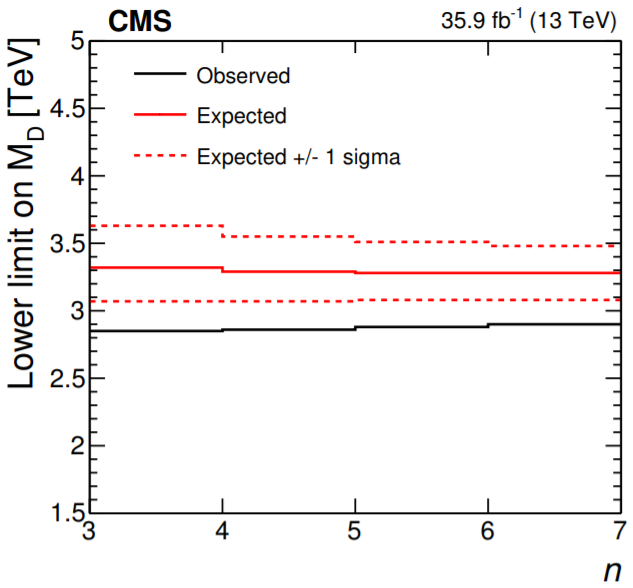
\includegraphics[width=0.42\textwidth]{Figures/add.pdf}
    \caption{
      Diagram illustrating ADD graviton emission resulting in a monophoton signature.
    }
    \label{fig:add_diagram}
  \end{center}
\end{figure}

\subsection{Previous searches} \label{sec:introduction_ADD_previous_searches}
For distances $r$ much larger than $R$, the effective gravitational potential in the ADD model has the $1/r$ form proposed by Isaac Newton (in the weak-field limit).
However, for $r \ll R$, the Newton's law potential is multiplied by $(R/r)^{n}$, leading to significant deviations from Newtonian gravitational behavior.
If $\mD \approx 1\unit{TeV}$ and $n = 1$, then to reproduce the observed value of \mPl, $R$ must be \textasciitilde$10^{13}\unit{cm}$, which
would result in noticeable differences in the orbits of the planets~\cite{ref:S0370-2693(98)00466-3}. The case $n = 2$ is disfavored by precision
measurements of Newton's law over distances on the order of 0.1\unit{mm}~\cite{ref:0264-9381/32/3/033001}.

As in the case of the aTGC model, collider limits
become strictly more stringent with increases in collider energy, starting from the LEP and moving up through the Tevatron to the LHC.
Representative curves from each of these are shown in Fig.~\ref{fig:add_noncollider_comparison}, which also shows that collider limits
on \mD\ dominate noncollider limits for $n \geq 3$. As with the DM simplified models, the strongest mono-X limits on the ADD model come from
the mono-$j/V$ channel, while the monophoton channel is the second most sensitive. The most stringent mono-$j/V$ limits from CMS exclude the ADD model
at 95\% CL for \mD\ up to 9.9\unit{TeV} when $n = 2$, and for \mD\ up to 5.3\unit{TeV} when $n = 6$~\cite{ref:PhysRevD.97.092005}.

\begin{figure}[hbtp]
  \begin{center}
    \includegraphics[width=0.90\textwidth]{Figures/add_noncollider_comparison_jpeg.jpg}
    \caption{
      Comparison of collider and noncollider limits on ADD model parameters, as shown in~\cite{ref:0264-9381/32/3/033001}.
      The marked points are monojet limits from the LEP~\cite{ref:9789812702227_0266}, Tevatron~\cite{ref:PhysRevLett.101.181602}, and LHC~\cite{ref:j.physletb.2011.10.006, ref:PhysRevLett.110.011802, ref:0264-9381/32/3/033001}.
      The Irvine~\cite{ref:PhysRevD.32.3084, ref:PhysRevLett.44.1645}, Washington~\cite{ref:PhysRevLett.98.021101}, and Stanford~\cite{ref:PhysRevD.78.022002} curves come from direct measurements of Newton's law.
      The Casimir curve~\cite{ref:0264-9381/32/3/033001} synthesizes of a range of  experimental results that constrain the existence of strong gravity using the Casimir force,
      and the pbar-HE curve~\cite{ref:epjconf/20146605021, ref:0264-9381/32/3/033001} comes from analyses of electron double scattering and exotic atom spectroscopy.
      The ADD model is excluded at 95\% CL or more in the shaded region.
    }
    \label{fig:add_noncollider_comparison}
  \end{center}
\end{figure}

Prior to the analysis presented in this thesis, the most stringent ADD limits in the monophoton final state were set in the last published results from CMS,
based on 12.9\fbinv\ of data collected in the first half of 2016~\cite{ref:JHEP10(2017)073}. The ADD model was excluded at 95\% CL for \mD\ up to 2.31\unit{TeV}
for $n = 3$, climbing to 2.49\unit{TeV} at $n = 6$, as shown in Fig.~\ref{fig:add_cms_earlylimits_MD}.

\begin{figure}[hbtp]
  \begin{center}
    \includegraphics[width=0.50\textwidth]{Figures/add_cms_earlylimits_MD.pdf}
    \caption{
    ADD limits based on CMS data from the first half of 2016 analyzed in the monophoton channel, as shown in~\cite{ref:JHEP10(2017)073}.
    Limits from the previous CMS monophoton analysis of 8\unit{TeV} data~\cite{ref:j.physletb.2016.01.057} are also shown.
    The ADD model for a given $n$ (specified by the left edge of each bin) is excluded at 95\% CL or more for \mD\ below the curves.
    }
    \label{fig:add_cms_earlylimits_MD}
  \end{center}
\end{figure}

None of these analyses report any significant evidence of BSM physics.
